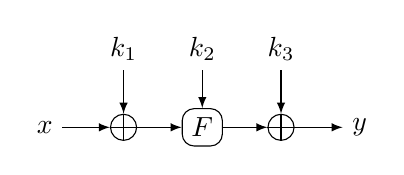
\begin{tikzpicture}
\node (x)  {$x$};
\node (xor) [right of=x, circle, draw] {};
\draw[-] (xor.north) -- (xor.south);
\draw[-] (xor.east) -- (xor.west);
\node (k1) [above of=xor] {$k_1$};
\node (f) [right of=xor, rounded corners=1ex, draw] {$F$};
\node (k2) [above of=f] {$k_2$};
\node (xor1) [right of=f, circle, draw] {};
\draw[-] (xor1.north) -- (xor1.south);
\draw[-] (xor1.east) -- (xor1.west);
\node (k3) [above of=xor1] {$k_3$};
\node (y)  [right of=xor1] {$y$};
\draw [-latex] (x) -- (xor);
\draw [-latex] (k1) -- (xor);
\draw [-latex] (xor) -- (f);
\draw [-latex] (k2) -- (f);
\draw [-latex] (f) -- (xor1);
\draw [-latex] (k3) -- (xor1);
\draw [-latex] (xor1) -- (y);
\end{tikzpicture}